% BerechnungVonGelichstromkreisen.tex

\section{Berechnung von Gleichstromkreisen}
\label{sec:BerechnungVonGleichstromkreisen}

\subsection{Einfache Schaltungen}
\label{sec:EinfacheSchaltungen}

\subsubsection{Serieschaltung von Widerst�nden}
\label{sec:SerieschaltungVonWiderst�nden}

\[
R=R_1+R_2+R_3+...
\]
\[
R=\sum_{i=1}^nR_i
\]

\subsubsection{Parallelschaltung von Widerst�nden}
\label{sec:ParallelschaltungVonWiderst�nden}
\[
\frac{1}{R}=\frac{1}{R_1}+\frac{1}{R_2}+\frac{1}{R_3}+...
\]
\[
G=G_1+G_2+G_3+...
\]
\[
G=\sum_{i=1}^nG_i
\]

\subsubsection{Stromteiler-Regel}
\label{sec:StromteilerRegel}

\begin{figure}[hb]
	\centering
%		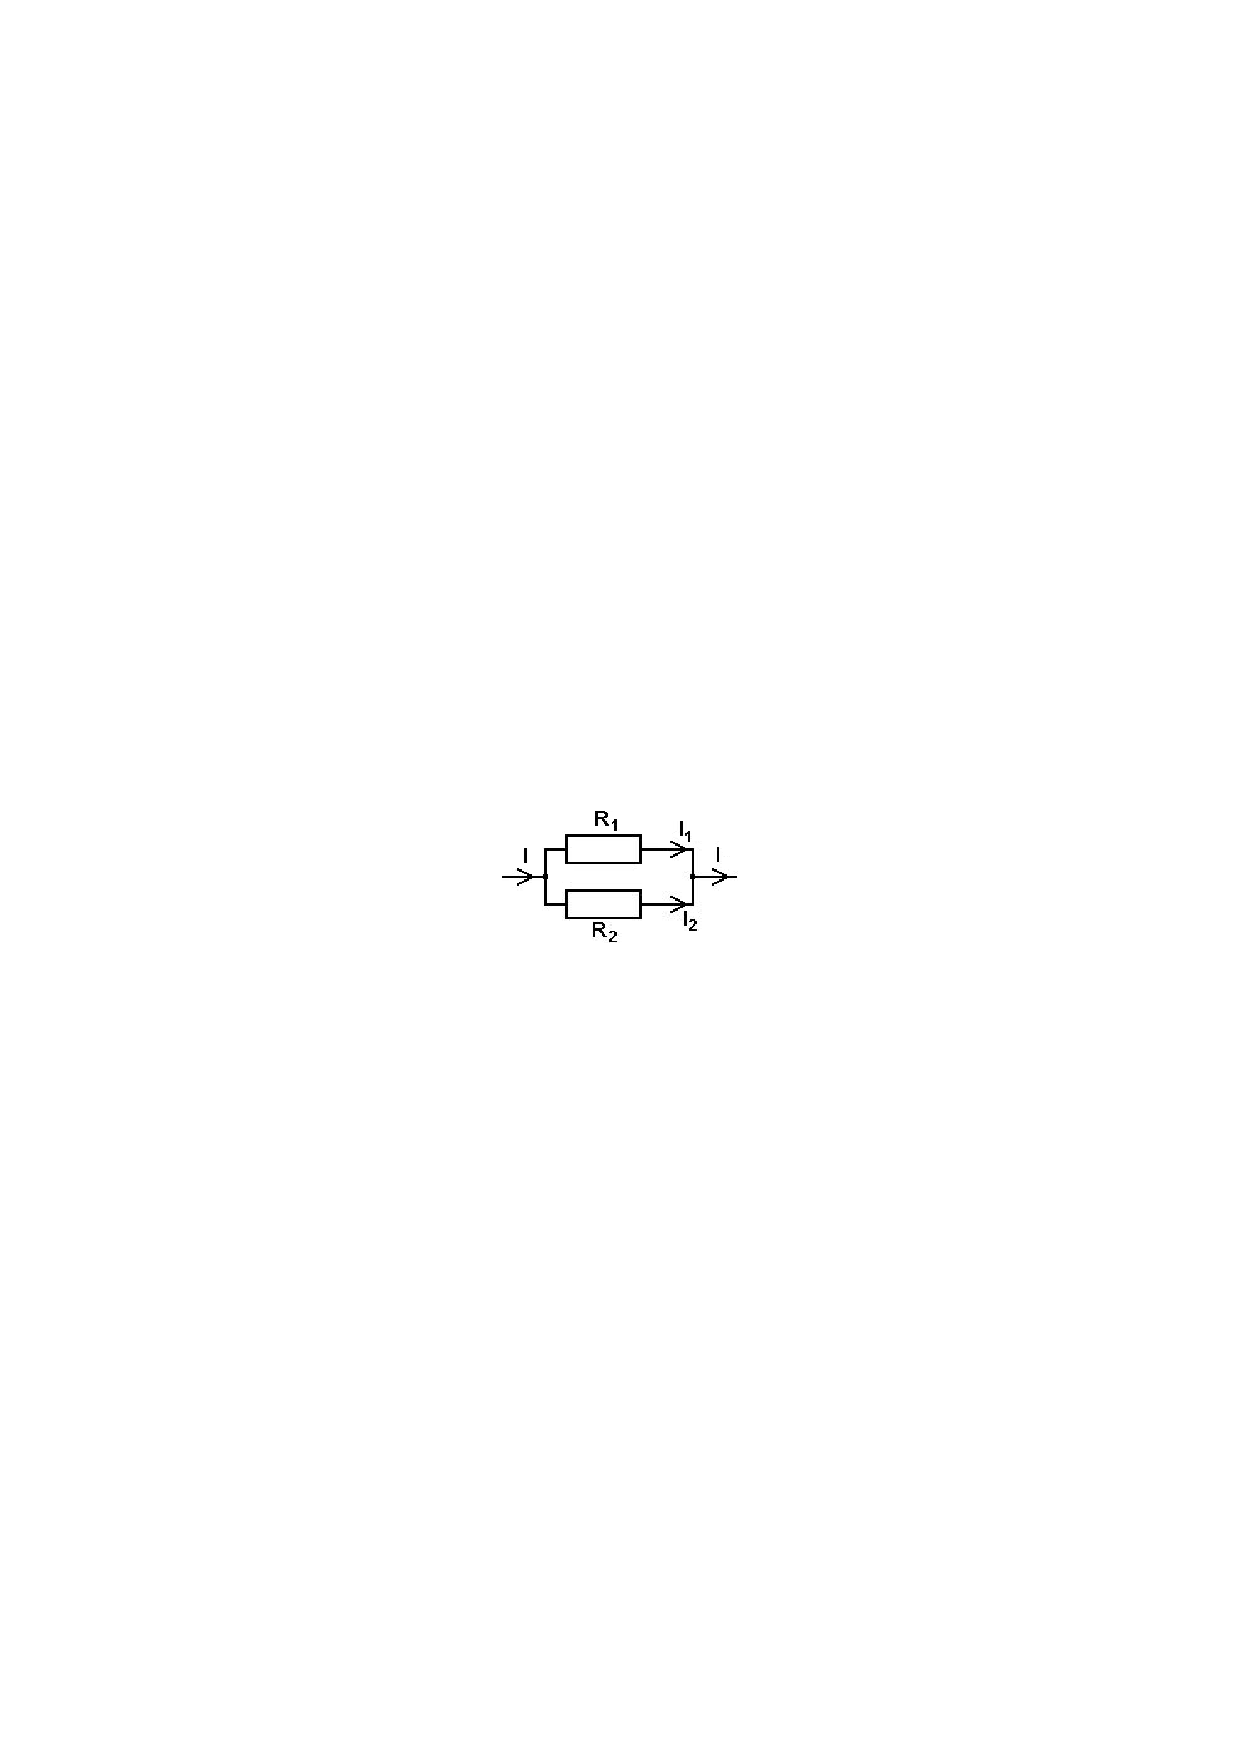
\includegraphics[width= 4 cm]{Grafiken/Stromteiler.png}
	\caption{Stromteiler}
	\label{fig:Stromteiler}
\end{figure}

\[
I \cdot R_{12} = I_1 \cdot R_1 = I_2 \cdot R_2
\]

\subsubsection{Spannungsteilerregel}
\label{sec:Spannungsteilerregel}
\begin{figure}[hb]
	\centering
%		\includegraphics[width=4 cm]{Grafiken/Spannungsteiler.png}
	\caption{Spannungsteiler}
	\label{fig:Spannungsteiler}
\end{figure}
\[
\frac{U_e}{U_a}=\frac{R_{12}}{R_2}
\]

\subsubsection{Stern- und Dreieckschaltungen}
\label{sec:SternDreieckSchaltungen}

\begin{figure}[htb]
	\centering
%		\includegraphics[width=8.00 cm]{Grafiken/Dreieck_Stern_Schaltung.png}
	\caption{a) Dreieckschaltung, b) Sternschaltung}
	\label{fig:Dreieckschaltung_Stern_Schaltung}
\end{figure}

\paragraph{Stern - Dreieck Umwandlung}
\label{sec:SternDreieckUmwandlung}

\[
R_{12}=R_1 +R_2+\frac{R_1\cdot R_2}{R_3}
\]
\[
R_{23}=R_2 +R_3+\frac{R_2\cdot R_3}{R_1}
\]
\[
R_{31}=R_3 +R_1+\frac{R_3\cdot R_1}{R_2}
\]

\paragraph{Dreieck - Stern Umwandlung}
\label{sec:DreieckSternUmwandlung}
%(Bild)
\[
R_1=\frac{R_{12} \cdot R_{31}}{R_{12}+R_{23}+R_{31}}
\]
\[
R_2=\frac{R_{23} \cdot R_{12}}{R_{12}+R_{23}+R_{31}}
\]

\[
R_3=\frac{R_{31} \cdot R_{23}}{R_{12}+R_{23}+R_{31}}
\] 

Bei Symmetrischer Schaltung mit $R_{12}=R_{23}=R_{31}=R_{\Delta}$
\[
R_\Yup =\frac{R_\Delta^2}{3 \cdot R_\Delta}=\frac{R_\Delta}{3}
\]
\subsection{Netzwerk-Analyse}
\label{sec:NetzwerkAnalyse}
\subsubsection{Knotenpotential-Verfahren}
\label{sec:KnotenpotentialVerfahren}
\subsubsection{Maschenstrom-Verfahren}
\label{sec:Maschenstromverfahren}
\subsubsection{�berlagerungssatz (Superposition)}
\label{sec:�berlagerungssatzSuperposition}
